\documentclass[11pt,a4paper]{article}
\usepackage[T1]{fontenc}
\usepackage[utf8]{inputenc}
\usepackage[french]{babel}
\usepackage{lmodern}
\usepackage{geometry}
\geometry{margin=2.3cm}
\usepackage{amsmath,amssymb,booktabs,array,multirow,tabularx}
\usepackage{graphicx}
\usepackage{float}
\usepackage{caption}
\captionsetup{font=small,labelfont=bf}
\usepackage{hyperref}
\usepackage{xurl}
\usepackage{xcolor}
\usepackage{fancyhdr}
\usepackage{enumitem}
\usepackage{tocloft}
\setlength{\cftbeforesecskip}{2pt}
\setlength{\cftbeforesubsecskip}{0pt}
\renewcommand{\cftsecafterpnum}{\hfill}
\hypersetup{colorlinks=true,linkcolor=blue!45!black,urlcolor=blue!45!black,citecolor=blue!45!black}
\pagestyle{fancy}
\fancyhf{}
\fancyhead[L]{\small Barrières tarifaires et exportations de tomates}
\fancyhead[R]{\small Data Science et commerce international}
\fancyfoot[C]{\thepage}
\setlength{\parskip}{0.35em}
\setlength{\parindent}{0pt}
\setlength{\emergencystretch}{2em}

\title{\textbf{Rapport de projet -- Data Science et commerce international}}
\author{Hiba Yacoubi \and Meriem Ninia}
\date{11 novembre 2026}

\begin{document}

\begin{titlepage}
\centering
{\Large L'École Nationale de Commerce et de Gestion de Settat (ENCG Settat) \par}
\vspace{0.6cm}
{\large Filière : Master Commerce International\par}
\vspace{0.15cm}
{\large Module : Data Science appliquée au commerce international\par}
\vspace{1.6cm}
{\Huge\bfseries Barrières tarifaires et exportations marocaines de tomates\par}
\vspace{0.4cm}
{\LARGE Droits NPF, concentration des marchés et flux, 2010--2023\par}
\vspace{0.8cm}
{\large Rapport scientifique de projet — Projet 35\par}
\vspace{1.4cm}
\begin{tabular}{rl}
Étudiante 1 : & Hiba Yacoubi \\
Étudiante 2 : & Meriem Ninia \\
Responsable : & A. Larhlimi \\
Année universitaire : & 2026--2027 \\
Date de remise : & 11 novembre 2026 \\
\end{tabular}
\end{titlepage}

\section*{Résumé}
\addcontentsline{toc}{section}{Résumé}

Ce projet décrit et classe les marchés de destination des exportations marocaines de
tomates fraîches (HS 0702) selon les droits de douane qui y sont appliqués, puis
quantifie la relation entre ces droits et les flux observés. Les données sont
\emph{entièrement réelles} et proviennent de quatre sources publiques : UN Comtrade
(506 observations, 2010--2023), la Banque mondiale (PIB), WITS/UNCTAD TRAINS (droits
NPF) et CEPII (distances).

Les exportations passent de 300 à 1\,140 millions de dollars, soit +280\,\%
(10,8\,\%/an). La France absorbe 66,4\,\% du total et les cinq premiers marchés
94,2\,\% : la concentration est le fait structurant du dossier. Quatre modèles ont été
comparés avec un découpage temporel strict (train 2010--2019, validation 2020--2021,
test 2022--2023). Le Random Forest obtient le meilleur $R^2$ hors échantillon
(0,286), devant Ridge (0,213) ; la baseline par la moyenne est à $-0{,}002$. Les
performances sont donc modestes, et nous l'assumons : deux variables ne suffisent pas à
expliquer la répartition des flux.

Le résultat le plus important est négatif et instructif : l'élasticité estimée au
droit NPF est \textbf{positive} ($+2{,}22$, IC 95\,\% $[+0{,}78\,;\,+3{,}65]$). Le
signe s'explique par la variable elle-même — les droits NPF les plus élevés sont ceux
de l'Union européenne, qui reçoit pourtant 83\,\% des flux grâce à l'accord
d'association UE-Maroc. Le NPF mesure donc l'appartenance au marché européen, pas une
barrière subie. Nous montrons que la question posée ne peut pas être tranchée avec les
données publiques accessibles, et nous expliquons précisément pourquoi.

\vspace{0.6em}
\noindent\textbf{Mots-clés :} barrières tarifaires, exportations marocaines, tomates,
droit NPF, concentration de marché, validation temporelle, Random Forest.

\begin{table}[H]
\centering
\caption{Chiffres clés du projet}\label{tab:chiffres}
\begin{tabular}{lr}
\toprule
Indicateur & Valeur \\
\midrule
Observations (Comtrade) & 506 \\
Partenaires déclarés & 80 nommés (83 codes) \\
Période couverte & 2010--2023 \\
Valeur cumulée exportée & 8,95 Md\$ \\
Croissance 2010--2023 & $+280$\,\% (CAGR 10,8\,\%) \\
Premier marché (France) & 66,4\,\% du total \\
Part du top 5 & 94,2\,\% \\
Observations avec droit NPF & 246 (48,6\,\%), 98,2\,\% de la valeur \\
Meilleur modèle (test) & Random Forest, $R^2 = 0{,}286$ \\
Élasticité au droit NPF & $+2{,}22$ $[+0{,}78\,;\,+3{,}65]$ \\
\bottomrule
\end{tabular}
\end{table}

\newpage
\tableofcontents
\newpage

\section{Introduction}\label{sec:intro}

\subsection{Contexte économique}

Le Maroc est un exportateur majeur de produits agricoles frais vers l'Europe. La
tomate (HS 0702) en est l'un des symboles : production de contre-saison, proximité
géographique, main-d'œuvre abondante et accès préférentiel au marché européen.

Cet accès repose sur l'accord d'association UE-Maroc entré en vigueur en 2000, qui
prévoit des contingents tarifaires préférentiels pour les fruits et légumes. La
contre-saison marocaine ne concurrence pas directement la production européenne
d'été, ce qui a permis à l'accord de fonctionner sans conflit majeur, malgré des
tensions récurrentes sur les volumes.

\subsection{Question de recherche}

Le catalogue du module (Projet 35) demande une \textbf{analyse descriptive et un
classement} : \emph{quels marchés pratiquent les droits les plus élevés pour ce
produit ?} La question causale — les droits réduisent-ils les flux ? — est une
extension naturelle, que nous traitons mais qui se heurte à une limite de données
détaillée plus bas.

\subsection{Hypothèses}

\begin{itemize}[leftmargin=1.2cm]
    \item \textbf{H1} — Les marchés appliquant des droits plus élevés attirent des
          flux plus faibles.
    \item \textbf{H2} — La proximité géographique et la taille du marché expliquent
          l'essentiel de la répartition des flux.
    \item \textbf{H3} — La relation tarif--exportation n'est pas linéaire.
\end{itemize}

\section{Données}\label{sec:data}

\subsection{Sources, période et unité d'analyse}

Les données sont extraites d'APIs publiques, sans clé d'accès. Chaque extraction
écrit un fichier de métadonnées contenant l'URL appelée, la date, les paramètres et la
licence.

\begin{table}[H]
\centering
\caption{Sources de données et traçabilité}\label{tab:sources}
\scriptsize
\setlength{\tabcolsep}{4pt}
\renewcommand{\arraystretch}{1.35}
\begin{tabularx}{\textwidth}{@{}>{\raggedright\arraybackslash}p{2.1cm}
                               >{\raggedright\arraybackslash}p{3.0cm}
                               >{\raggedright\arraybackslash}X
                               >{\raggedright\arraybackslash}p{2.2cm}@{}}
\toprule
\textbf{Source} & \textbf{Contenu} & \textbf{Endpoint appelé} & \textbf{Licence} \\
\midrule
UN Comtrade & Exportations Maroc, HS 0702, 2010--2023 &
\url{https://comtradeapi.un.org/public/v1/preview/C/A/HS} &
Données publiques ONU \\
Banque mondiale (WDI) & PIB courant \texttt{NY.GDP.MKTP.CD} &
\url{https://api.worldbank.org/v2/country/{iso3}/indicator/NY.GDP.MKTP.CD} &
CC BY 4.0 \\
WITS / UNCTAD TRAINS & Droits NPF HS 070200 &
\url{https://wits.worldbank.org/API/V1/SDMX/V21/datasource/TRN/} &
CC BY 4.0 \\
CEPII & Distances bilatérales depuis le Maroc &
\url{https://www.cepii.fr/distance/dist_cepii.zip} &
Citation CEPII \\
\bottomrule
\end{tabularx}
\end{table}

\textbf{Période :} 2010 à 2023 (14 années).

\textbf{Unité d'analyse :} paire \emph{pays importateur $\times$ année}.

\textbf{Volume :} 506 observations, 83 codes partenaires dont 80 nommés.

\textbf{Extraction :} 11 novembre 2026. Les réponses HTTP sont mises en cache
(\texttt{data/raw/api\_cache/}, \texttt{data/raw/wits\_cache/}) : relancer un script ne
re-sollicite pas les serveurs.

\subsection{Dictionnaire des variables}

Le dictionnaire complet, séparé par source, figure dans
\texttt{DICTIONNAIRE\_VARIABLES.md}. Le tableau~\ref{tab:variables} en donne l'essentiel.

\begin{table}[H]
\centering
\caption{Variables principales, par source}\label{tab:variables}
\small
\begin{tabular}{llll}
\toprule
\textbf{Variable} & \textbf{Source} & \textbf{Unité} & \textbf{Rôle} \\
\midrule
\texttt{period} & Comtrade & année & Index temporel \\
\texttt{partnerName} & Comtrade (référentiel) & texte & Pays importateur \\
\texttt{primaryValue} & Comtrade & USD & \textbf{Cible} \\
\texttt{netWgt} & Comtrade & kg & Cible alternative \\
\texttt{gdp\_partner\_usd} & Banque mondiale & USD & Contrôle \\
\texttt{distance\_km\_cepii} & CEPII & km & Contrôle (constante par pays) \\
\texttt{tariff\_npf\_pct} & WITS & \% & Droit NPF (voir §\ref{sec:limite-npf}) \\
\texttt{log\_value} & calculée & -- & $\ln(\texttt{primaryValue})$ \\
\texttt{log\_gdp} & calculée & -- & $\ln(\texttt{gdp\_partner\_usd})$ \\
\texttt{log\_distance} & calculée & -- & $\ln(\texttt{distance\_km\_cepii})$ \\
\bottomrule
\end{tabular}
\end{table}

\subsection{Qualité et préparation}

\textbf{Valeurs manquantes.} Aucune imputation n'a été faite. Les manquants sont
signalés et documentés :

\begin{table}[H]
\centering
\caption{Couverture des variables clés}\label{tab:couverture}
\small
\begin{tabular}{lrrl}
\toprule
\textbf{Variable} & \textbf{Renseignées} & \textbf{Taux} & \textbf{Cause} \\
\midrule
\texttt{primaryValue} & 506 / 506 & 100,0\,\% & -- \\
\texttt{gdp\_partner\_usd} & 434 / 506 & 85,8\,\% & Partenaires hors référentiel WDI \\
\texttt{distance\_km\_cepii} & 491 / 506 & 97,0\,\% & 3 codes non résolus, pays absents de CEPII \\
\texttt{tariff\_npf\_pct} & 246 / 506 & 48,6\,\% & 10 déclarants WITS seulement \\
\bottomrule
\end{tabular}
\end{table}

\textbf{Doublons.} Aucun doublon sur la paire (partenaire, année).

\textbf{Cohérence.} \texttt{flowCode} vaut \texttt{X} partout, \texttt{reporterCode}
vaut 504 (Maroc), \texttt{cmdCode} vaut \texttt{0702}.

\textbf{Valeurs extrêmes.} 83 observations sortent de l'intervalle
$[q_1 - 1{,}5\,IQR\,;\,q_3 + 1{,}5\,IQR]$ sur \texttt{primaryValue}. Ce sont de très
petits flux réels (à partir de 2 USD), pas des erreurs de saisie. Les supprimer
biaiserait la répartition géographique : elles sont conservées.

\textbf{Transformations.} Logarithmes naturels calculés uniquement quand la valeur est
strictement positive. Le taux de croissance n'est calculé que sur des années
consécutives (\texttt{intervalle\_annees == 1}) : sans cette précaution, un pays
observé en 2010 puis en 2014 produisait une « croissance » de +5\,543\,\% dépourvue de
sens.

\subsection{Limite majeure : le droit NPF n'est pas le droit subi}\label{sec:limite-npf}

L'API WITS renvoie le droit \textbf{NPF} (\emph{Most Favoured Nation}) : le tarif
appliqué aux pays \emph{sans} accord préférentiel, en moyenne simple sur les lignes
HS6. Or le Maroc bénéficie de l'accord d'association UE-Maroc : ses tomates entrent en
franchise ou à taux réduit, bien en dessous du NPF.

L'API ne fournit pas le taux préférentiel Maroc : la requête
\texttt{partner/504} renvoie 404 pour la plupart des déclarants. Nous avons donc
explicitement choisi de nommer la variable \texttt{tariff\_npf\_pct} et non
\texttt{tariff\_rate}, pour qu'aucun lecteur ne puisse la confondre avec le tarif
réellement payé.

\textbf{Conséquence méthodologique.} Toute élasticité estimée sur cette variable
mesure un effet de \emph{sélection des marchés}, pas un effet causal du tarif subi.
Nous verrons en §\ref{sec:elasticite} que cette limite n'est pas théorique : elle
inverse le signe du coefficient attendu.

\section{Analyse exploratoire}\label{sec:eda}

Cinq figures commentées constituent le Jalon 1. Les interprétations sont générées par
le script à partir des chiffres mesurés, puis relues.

\subsection{Évolution des exportations}

\begin{figure}[H]
\centering
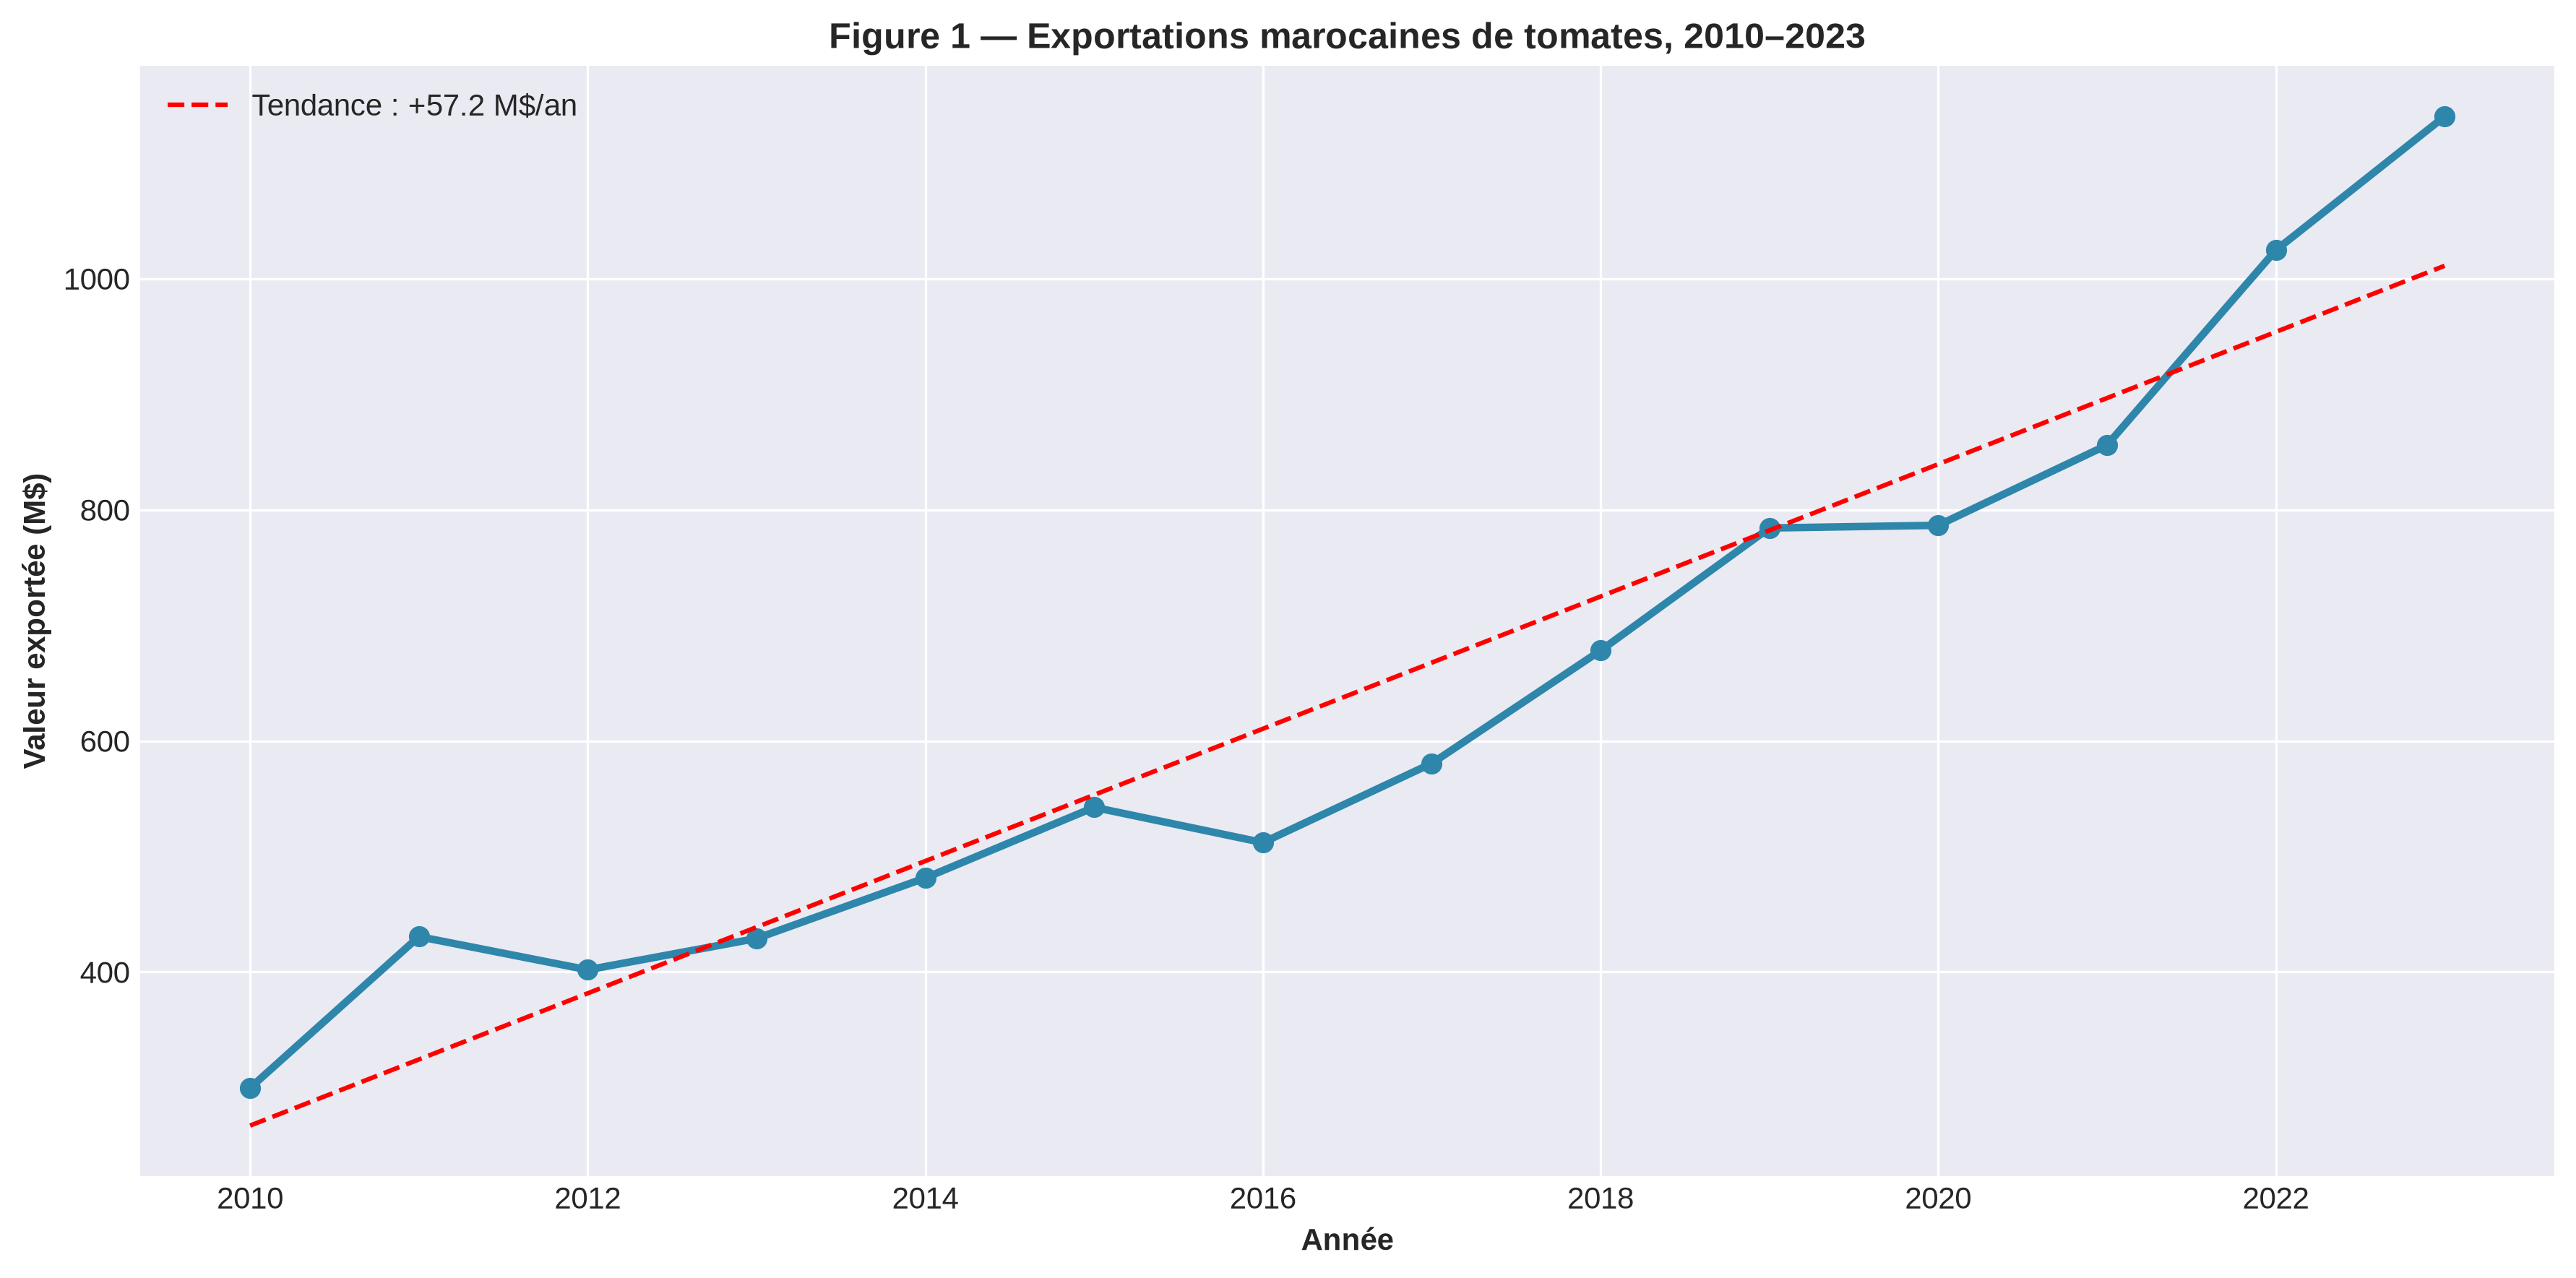
\includegraphics[width=0.85\linewidth]{../figures/fig1_evolution_temporelle.png}
\caption{Exportations marocaines de tomates, 2010--2023 (M\$).}
\label{fig:evolution}
\end{figure}

Les exportations passent de 299,7 M\$ en 2010 à 1\,140,3 M\$ en 2023, soit
$+280$\,\%, ou 10,8\,\%/an en moyenne. La progression est presque continue. Le choc
COVID de 2020 ne produit pas de rupture : l'année (786,5 M\$) reste au-dessus de 2019
(784,2 M\$). La demande européenne en contre-saison a donc résisté à la pandémie.

\subsection{Concentration des destinations}

\begin{figure}[H]
\centering
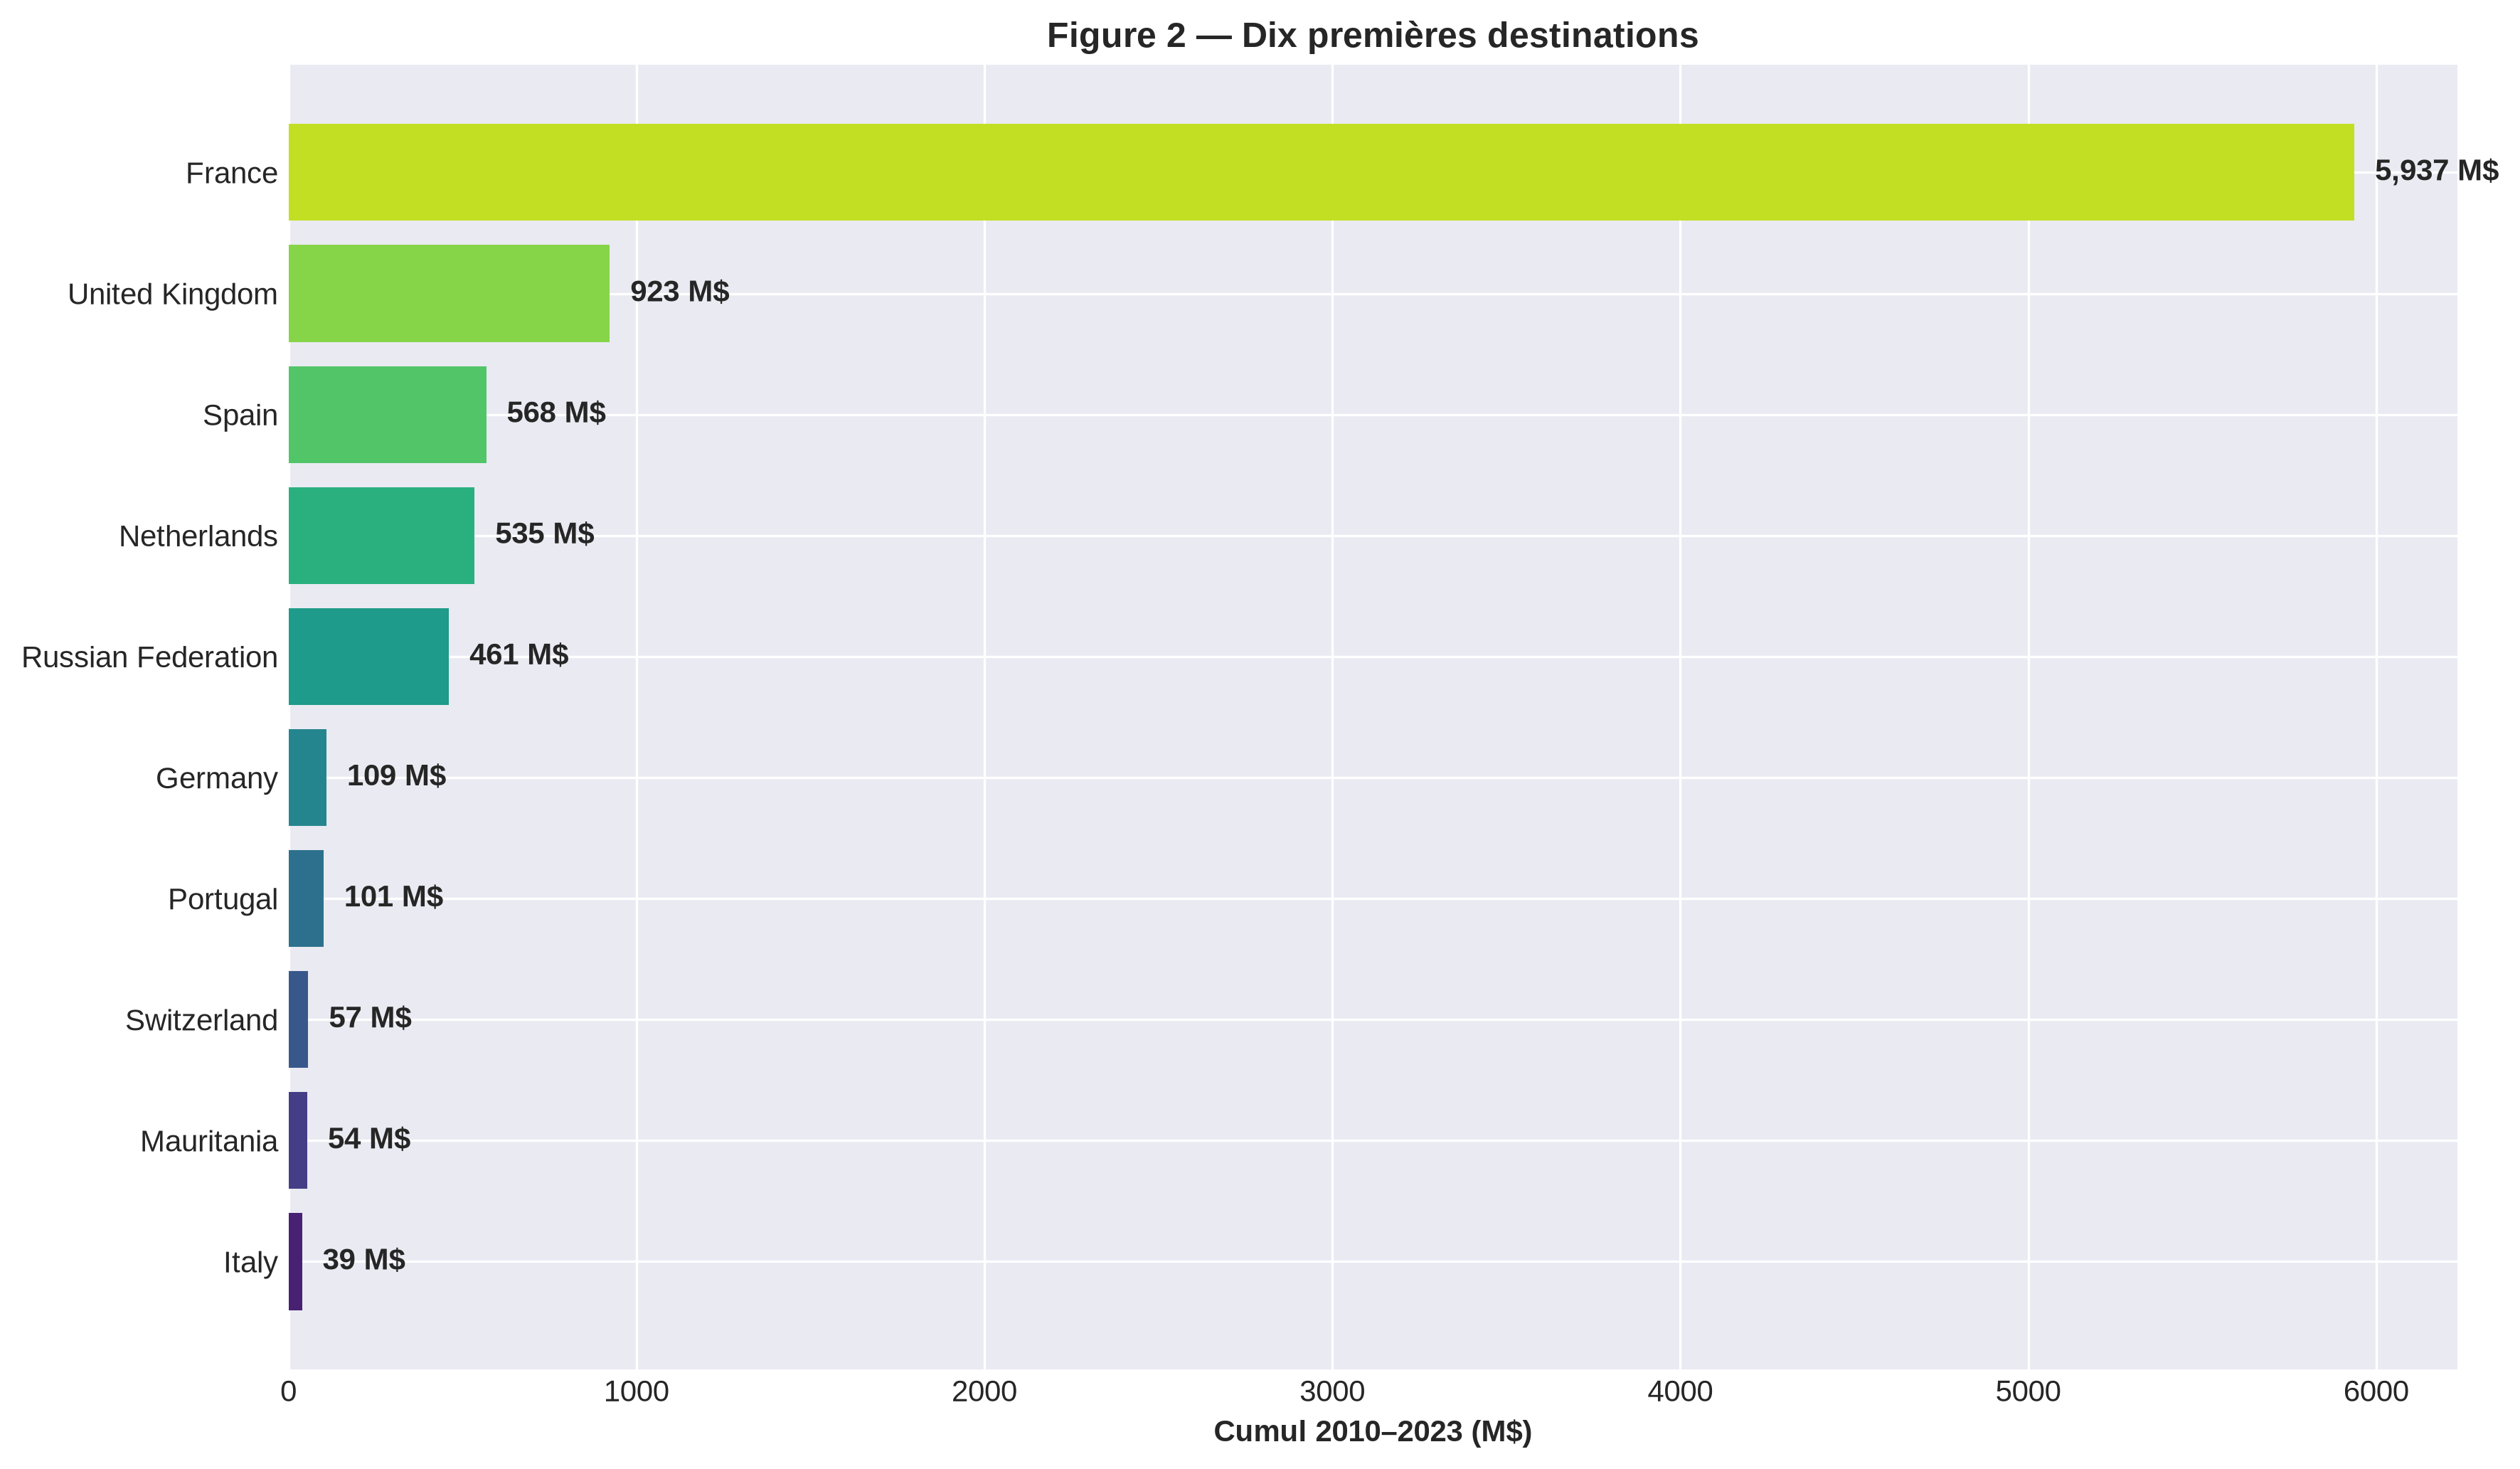
\includegraphics[width=0.85\linewidth]{../figures/fig2_top10_destinations.png}
\caption{Dix premières destinations, valeur cumulée 2010--2023.}
\label{fig:top10}
\end{figure}

La France domine avec 5\,937 M\$ cumulés, soit \textbf{66,4\,\%} du total. Le
Royaume-Uni suit à 10,3\,\%, puis l'Espagne (6,4\,\%), les Pays-Bas (6,0\,\%) et la
Russie (5,2\,\%). Les cinq premiers marchés concentrent \textbf{94,2\,\%} des
exportations.

Cette concentration est le fait marquant du dossier. Elle combine proximité
géographique, communauté de langue et de diaspora, et accès préférentiel au marché
européen. Elle constitue aussi la principale vulnérabilité : une perturbation sur un
seul marché affecterait la majorité des flux.

\subsection{Droits NPF et flux}

\begin{figure}[H]
\centering
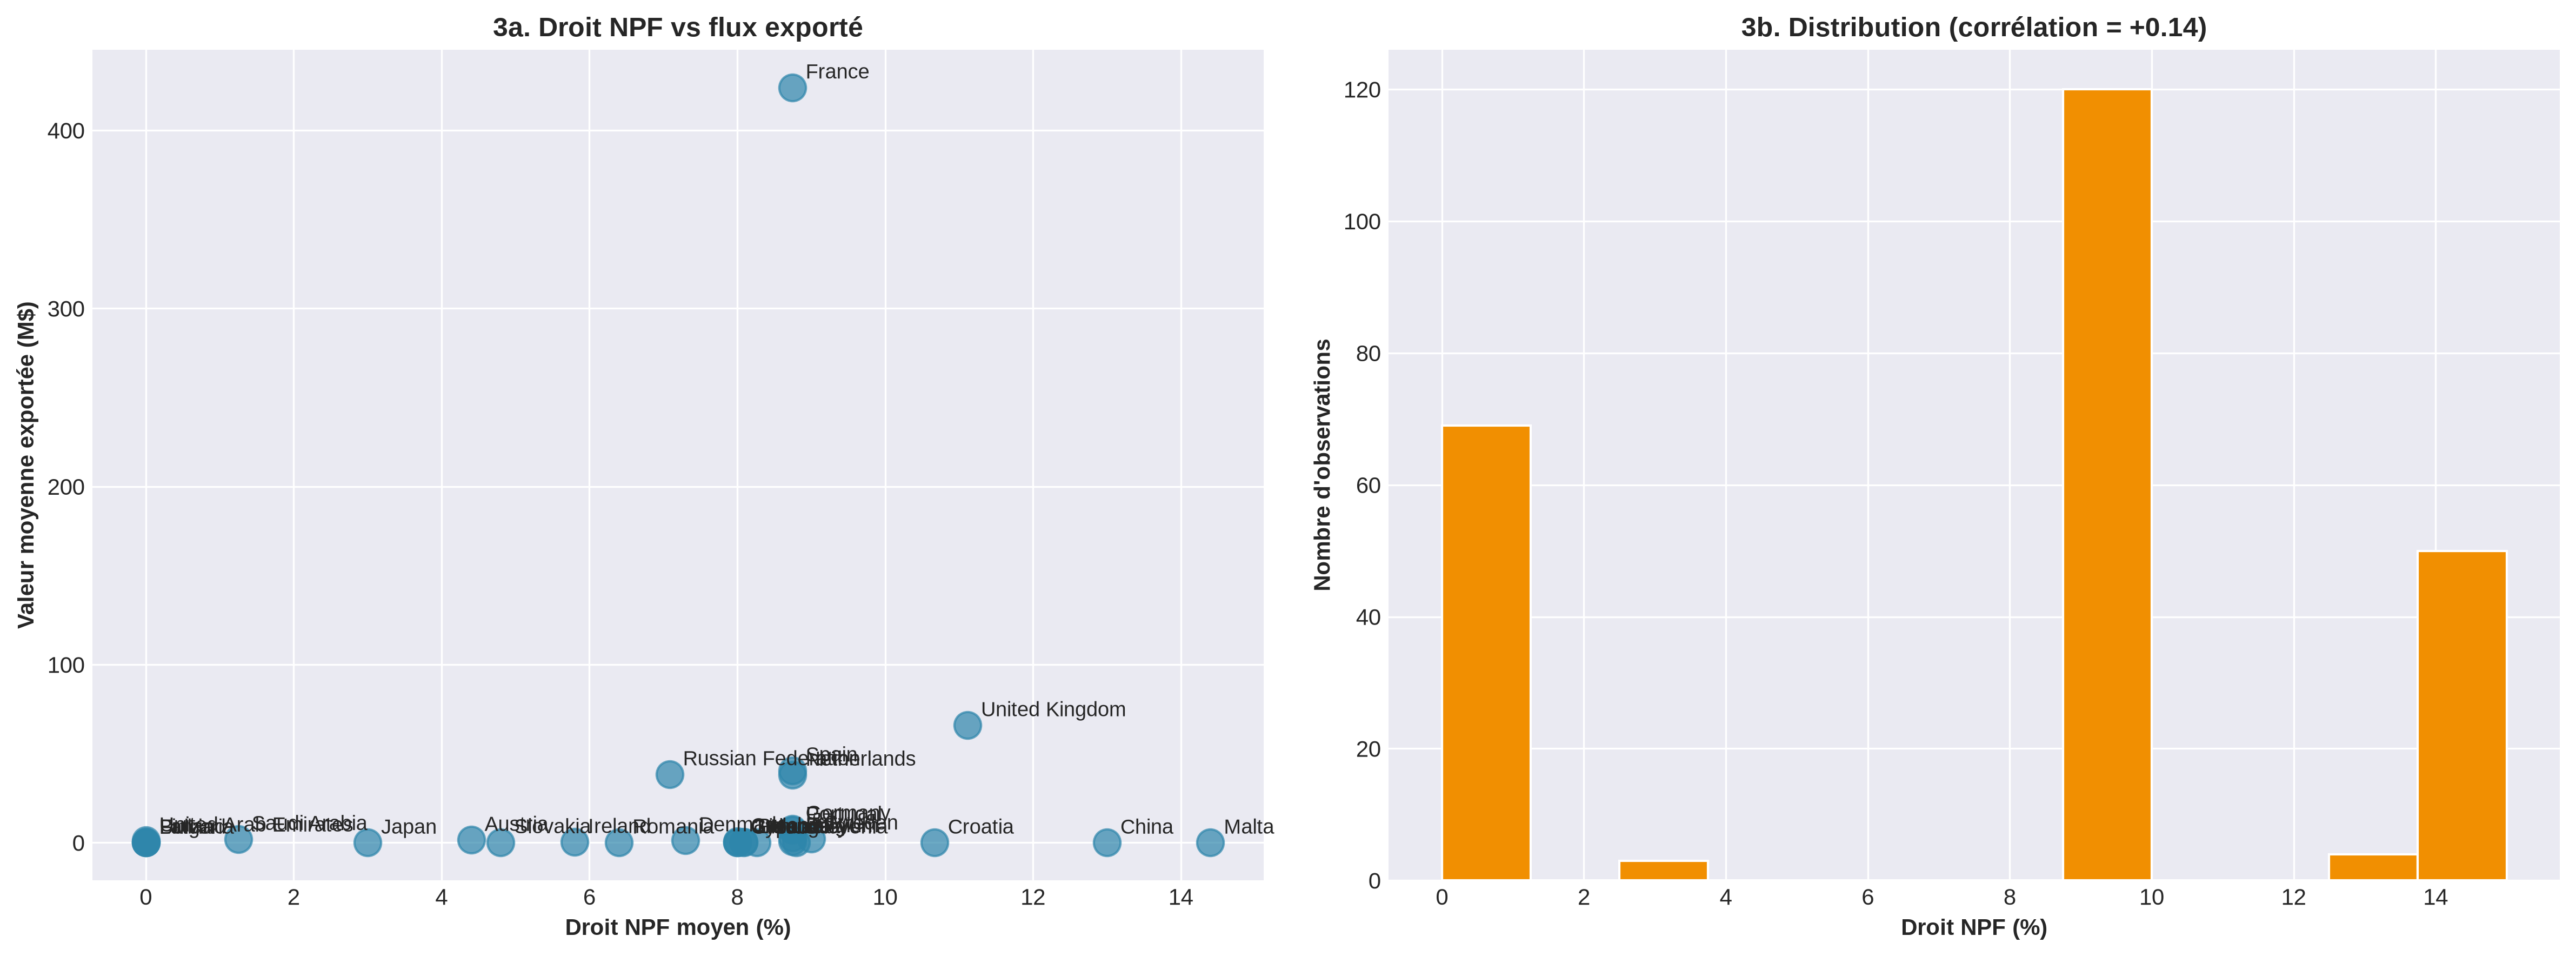
\includegraphics[width=0.85\linewidth]{../figures/fig3_correlation_tarifs.png}
\caption{Droit NPF moyen par partenaire et distribution des droits.}
\label{fig:correlation}
\end{figure}

La corrélation entre droit NPF moyen et valeur moyenne exportée est de
$\mathbf{+0{,}14}$ sur 31 partenaires couverts. Elle est faible et de signe positif :
\emph{contrairement à l'intuition, les marchés à NPF élevé ne reçoivent pas moins de
flux}. Ce résultat, qui contredit H1, s'explique par la structure de la variable et
sera repris en §\ref{sec:elasticite}.

La distribution des droits n'est pas continue : elle se concentre sur quelques
paliers (0\,\%, 8,8\,\%, 14,4\,\%), correspondant aux lignes tarifaires saisonnières
de l'Union européenne. Cette granularité limite fortement la puissance d'une
estimation par régression : l'essentiel de la variation est un effet de régime, pas
un gradient.

\subsection{Zones et structure du marché}

\begin{figure}[H]
\centering
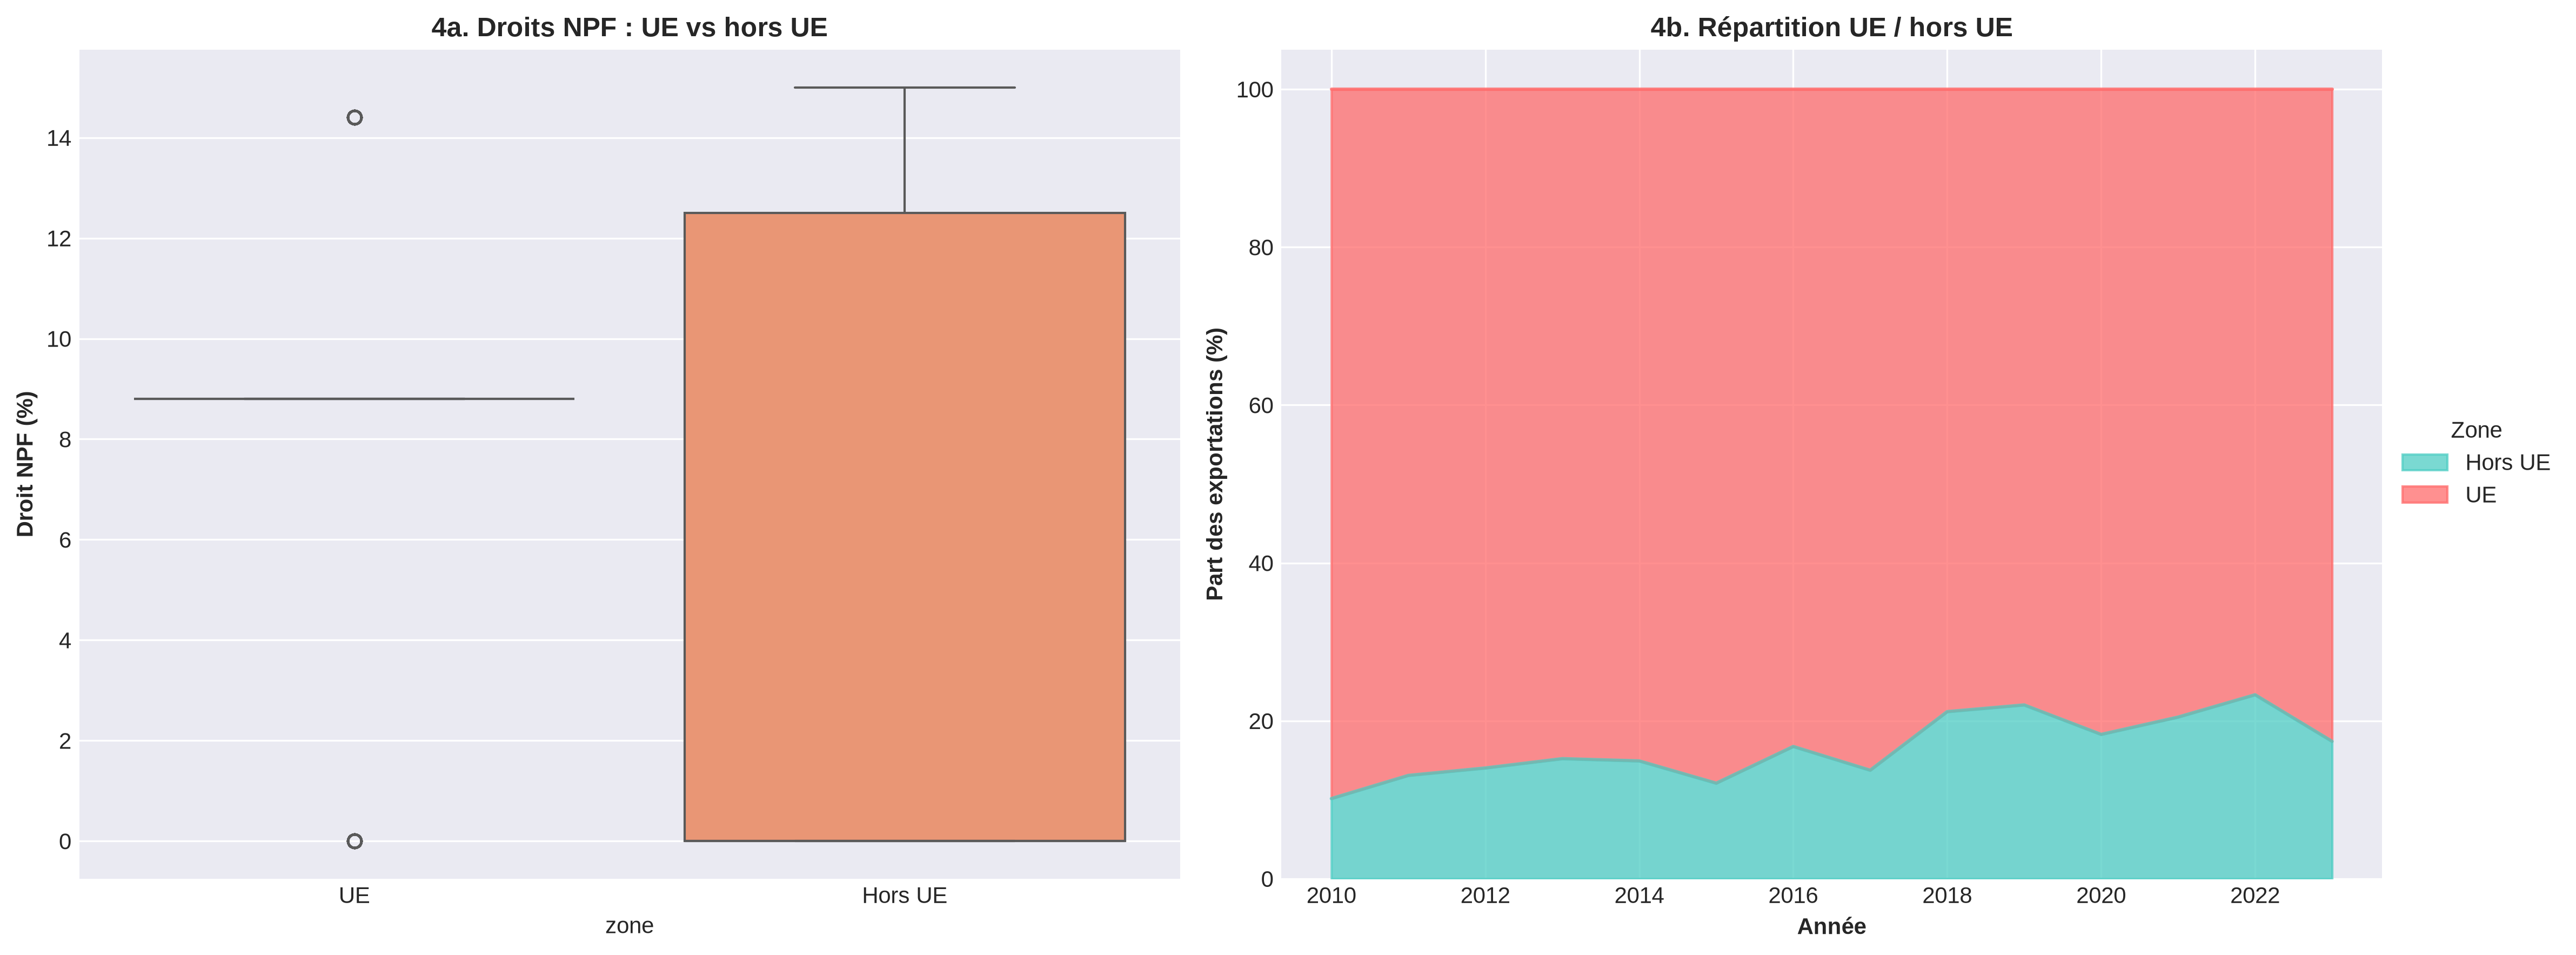
\includegraphics[width=0.85\linewidth]{../figures/fig4_distribution_tarifs.png}
\caption{Droits NPF UE / hors UE et répartition des exportations par zone.}
\label{fig:distribution}
\end{figure}

Les droits NPF de l'UE sont stables, avec une médiane à 8,8\,\%, mais ils couvrent
une plage de 0 à 14,4\,\% selon la saison. Les pays hors UE sont plus dispersés
(Russie jusqu'à 15\,\%, Émirats à 0\,\%). L'UE absorbe en moyenne
\textbf{83,4\,\%} de la valeur exportée sur la période. La part hors UE progresse
cependant, portée par le Royaume-Uni et la Russie.

\subsection{Dynamiques et concentration}

\begin{figure}[H]
\centering
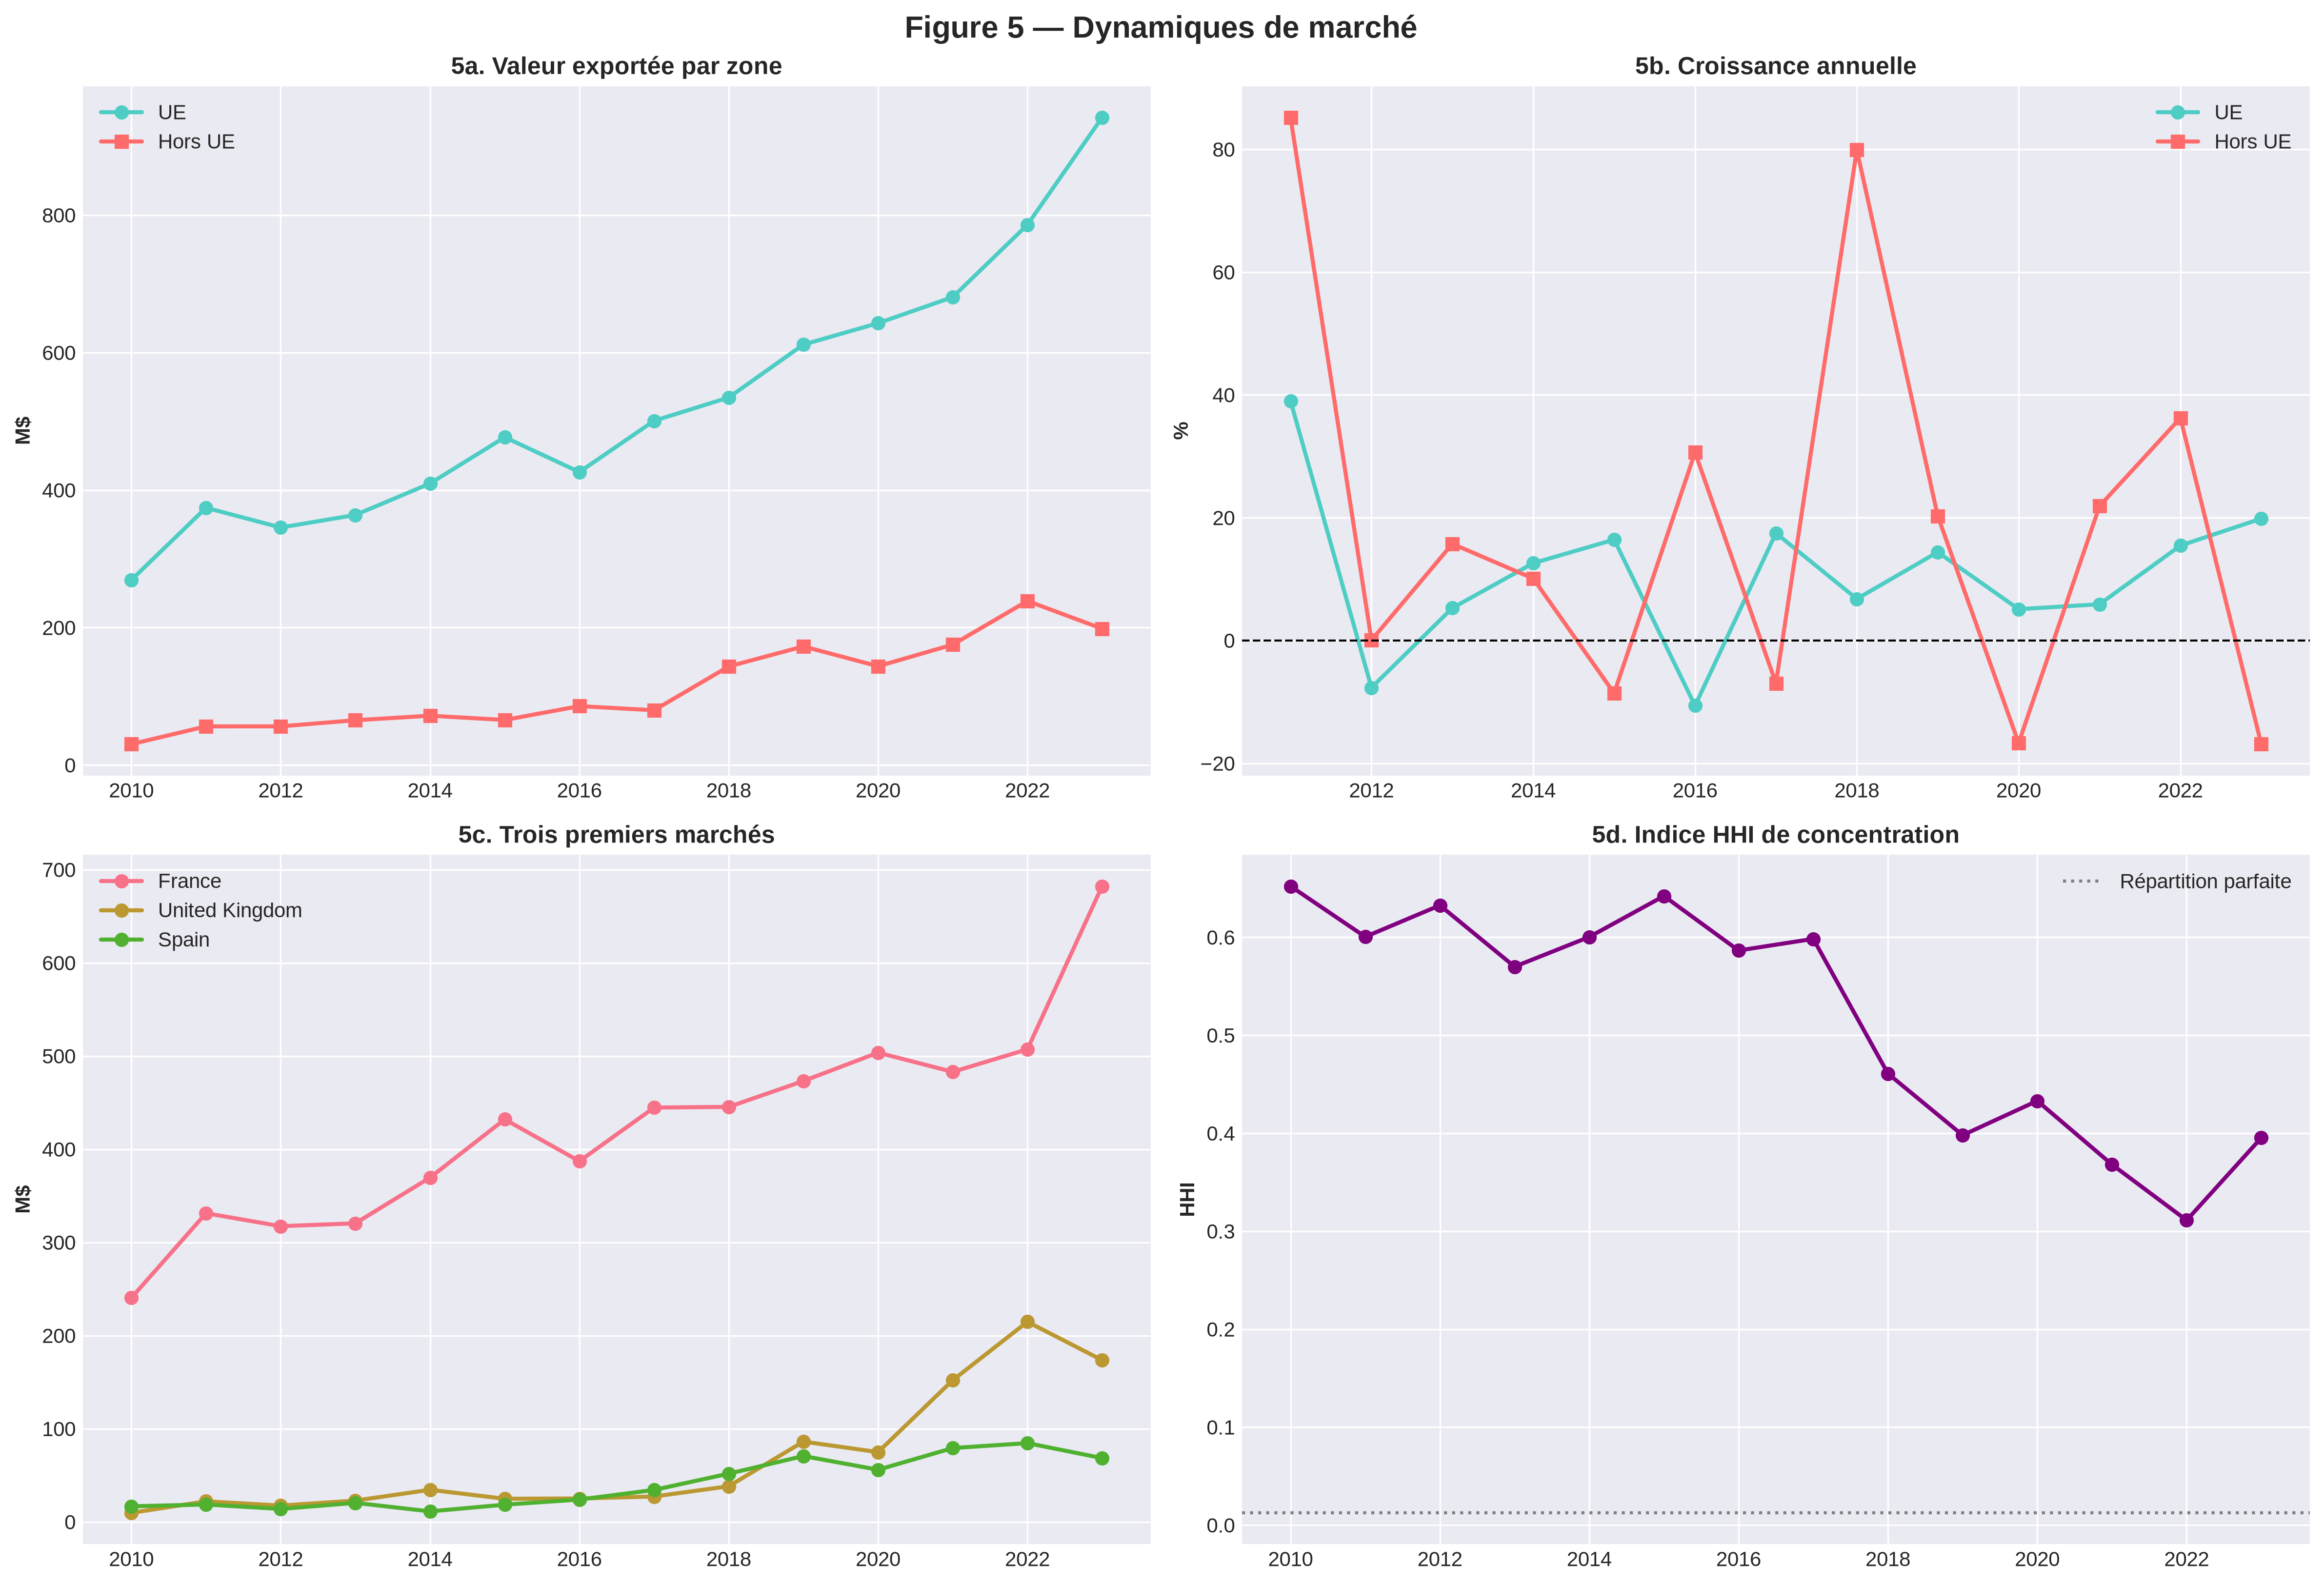
\includegraphics[width=0.85\linewidth]{../figures/fig5_series_temporelles.png}
\caption{Séries par zone, croissance annuelle, trois premiers marchés et indice HHI.}
\label{fig:series}
\end{figure}

L'indice Herfindahl-Hirschman passe de \textbf{0,652} en 2010 à \textbf{0,395} en
2023, pour une valeur de 0,013 correspondant à une répartition parfaitement égale. La
concentration diminue donc, mais reste trente fois supérieure à celle d'un marché
uniforme. Elle est structurelle et ne se corrige pas spontanément.

\section{Méthodologie}\label{sec:method}

\subsection{Découpage temporel}

La validation temporelle est obligatoire pour toute prévision : le modèle ne doit
jamais voir le futur. Le découpage est strict, sans mélange.

\begin{table}[H]
\centering
\caption{Découpage temporel du jeu de modélisation}\label{tab:split}
\begin{tabular}{llrl}
\toprule
\textbf{Jeu} & \textbf{Période} & \textbf{Observations} & \textbf{Usage} \\
\midrule
Train & 2010--2019 & 272 & Apprentissage \\
Validation & 2020--2021 & 71 & Choix des hyperparamètres \\
Test & 2022--2023 & 84 & Évaluation finale, une seule fois \\
\bottomrule
\end{tabular}
\end{table}

427 observations sur 506 sont modélisables (après suppression des manquants sur la
cible et les deux variables explicatives).

\subsection{Variables retenues et variables écartées}

\textbf{Retenues :} \texttt{log\_gdp} (taille du marché) et \texttt{log\_distance}
(coût de transport).

\textbf{Écartées, avec justification :}

\begin{itemize}[leftmargin=1.2cm]
    \item \texttt{trend} — un modèle à arbres ne sait pas extrapoler une tendance.
          Avec un découpage temporel, il plafonne à la dernière valeur vue à
          l'entraînement. La variable introduisait un biais, pas une information.
    \item \texttt{eu\_member} / \texttt{preferential\_agreement} — redondants avec
          l'effet fixe pays, et non sourcés dans la version précédente du projet.
    \item \texttt{tariff\_npf\_pct} — couverture de 48,6\,\% des observations.
          L'inclure dans le modèle principal aurait réduit l'échantillon de moitié et
          mélangé deux questions. Il fait l'objet d'une régression dédiée
          (§\ref{sec:elasticite}).
    \item \texttt{high\_tariff}, \texttt{lag\_weight}, \texttt{region} — dérivées de
          variables qui n'existaient pas réellement, ou jamais produites par le
          pipeline. Supprimées plutôt que fabriquées.
\end{itemize}

\subsection{Modèles}

\textbf{Baseline — moyenne historique.} $\widehat{y}_i = \bar{y}_{\text{train}}$.
Référence minimale : tout modèle doit faire mieux.

\textbf{Régression simple (PIB).}
$\log(\text{export}_i) = \beta_0 + \beta_1 \log(\text{PIB}_i) + \epsilon_i$.
Référence interprétable sur une seule variable.

\textbf{Ridge.} Régression linéaire régularisée, avec standardisation préalable.
L'hyperparamètre $\alpha$ est choisi sur le jeu de validation parmi
$\{0{,}01\,;\,0{,}1\,;\,1\,;\,10\,;\,100\}$.

\textbf{Random Forest.} Forêt d'arbres décisionnels. Grille de recherche sur
validation : \texttt{n\_estimators} $\in \{100, 300\}$, \texttt{max\_depth}
$\in \{3, 5, 8\}$, \texttt{min\_samples\_leaf} $\in \{1, 5\}$.

\subsection{Métriques}

\begin{align}
\mathrm{MAE} &= \frac{1}{n}\sum_{i=1}^{n}\left|y_i-\widehat{y}_i\right| \\
\mathrm{RMSE} &= \sqrt{\frac{1}{n}\sum_{i=1}^{n}(y_i-\widehat{y}_i)^2} \\
R^2 &= 1 - \frac{\sum_{i}(y_i-\widehat{y}_i)^2}{\sum_{i}(y_i-\bar{y})^2}
\end{align}

Les métriques portent sur $\log(\text{valeur})$ : une MAE de 1 correspond environ à
un facteur $e \approx 2{,}7$ d'erreur multiplicative.

\section{Résultats}\label{sec:results}

\subsection{Comparaison des modèles}

\begin{table}[H]
\centering
\caption{Performances sur validation (2020--2021) et test (2022--2023)}\label{tab:performances}
\small
\begin{tabular}{lrrrrr}
\toprule
\textbf{Modèle} & \textbf{MAE val} & \textbf{$R^2$ val} &
\textbf{MAE test} & \textbf{RMSE test} & \textbf{$R^2$ test} \\
\midrule
Baseline (moyenne) & -- & -- & 3,519 & 4,318 & $-0{,}002$ \\
Régression simple (PIB) & 2,538 & 0,228 & 3,152 & 4,309 & 0,002 \\
Ridge ($\alpha=1$) & 2,337 & 0,382 & 2,887 & 3,825 & 0,213 \\
\textbf{Random Forest (300, 8, 1)} & \textbf{1,878} & \textbf{0,545} &
\textbf{2,738} & \textbf{3,644} & \textbf{0,286} \\
\bottomrule
\end{tabular}
\end{table}

Le Random Forest est le meilleur modèle sur les deux jeux, avec un $R^2$ de 0,286 sur
le test. Ridge suit à 0,213. La régression sur le PIB seul ne fait pratiquement pas
mieux que la baseline (0,002 contre $-0,002$), ce qui indique que la taille du marché,
prise isolément, n'explique presque rien dans cet échantillon.

\textbf{Lecture honnête.} Un $R^2$ de 0,286 signifie que le modèle laisse 71\,\% de la
variance inexpliquée. Deux variables ne suffisent pas à décrire la répartition des
flux : il manque les prix, les coûts logistiques, les quotas, la saisonnalité et les
relations commerciales historiques. Nous ne présentons donc pas ce modèle comme
prédictif, mais comme un \emph{banc d'essai méthodologique} : il montre que la
validation temporelle fonctionne et que la géographie porte un signal réel, sans
prétendre épuiser le sujet.

\begin{figure}[H]
\centering
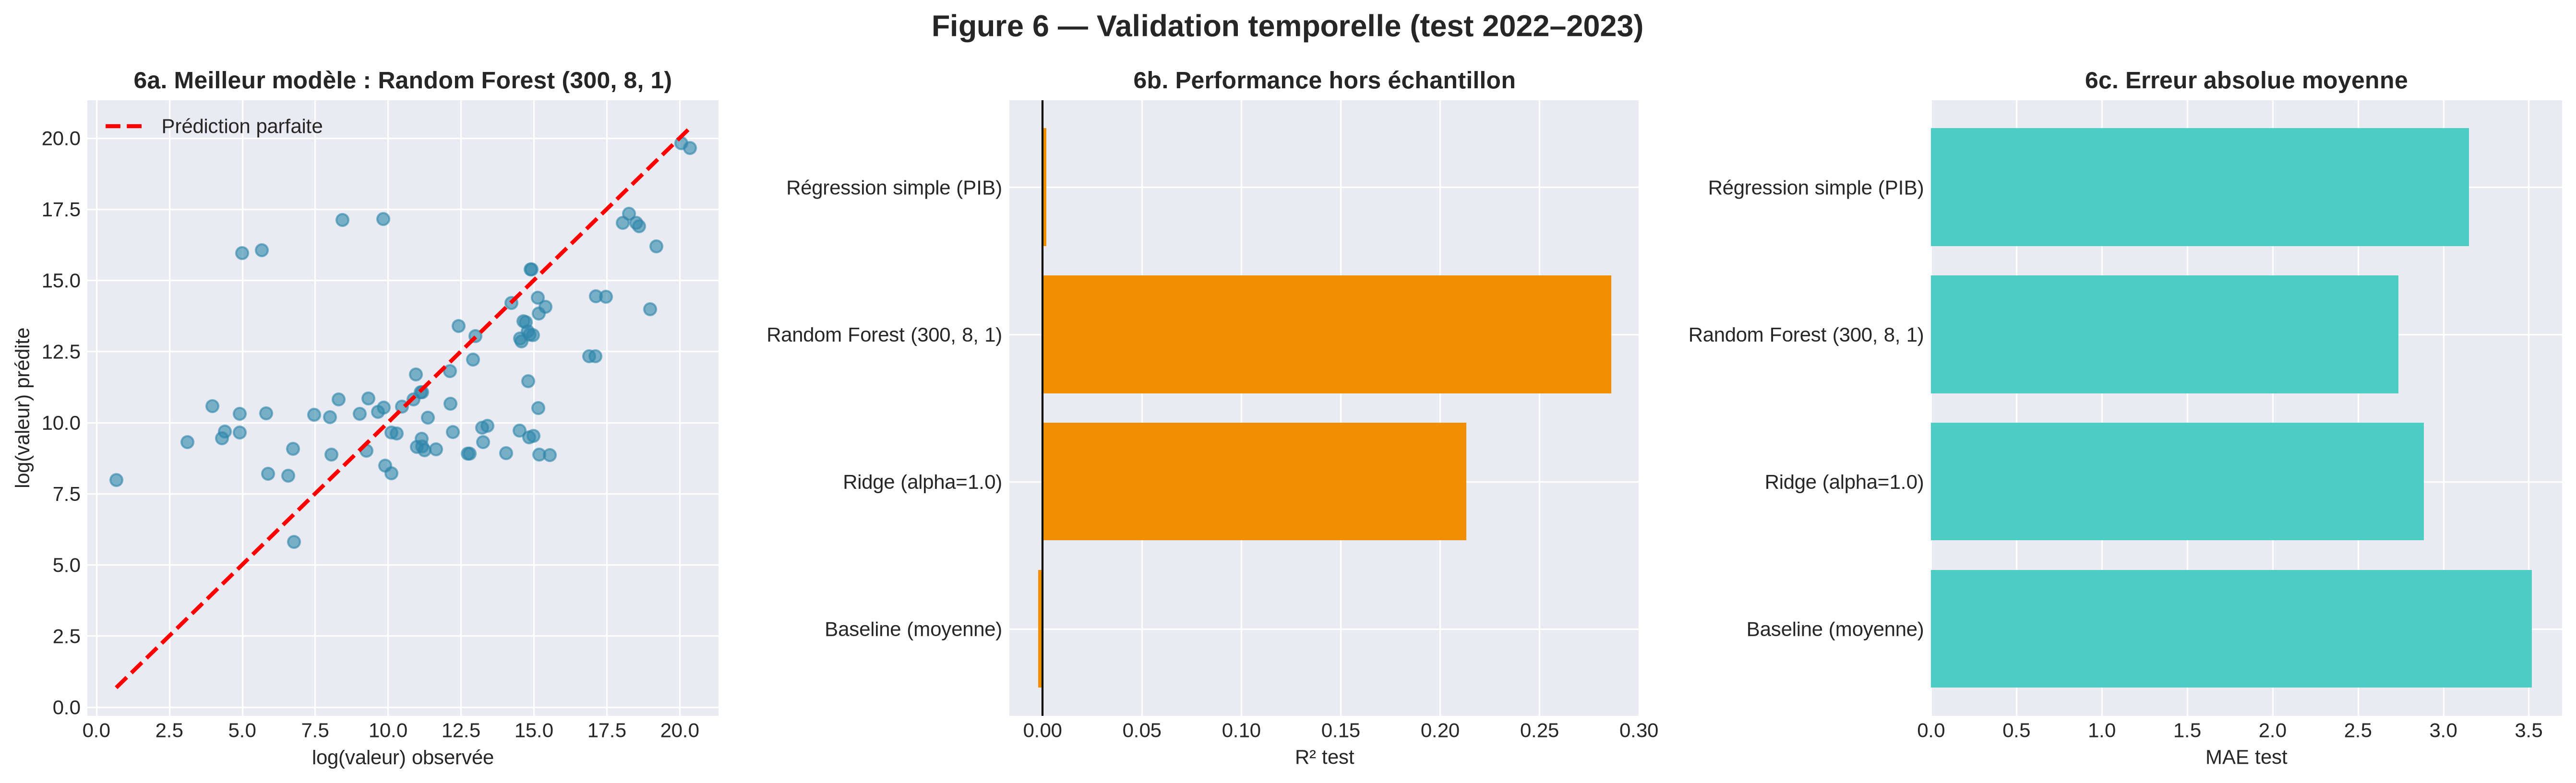
\includegraphics[width=0.95\linewidth]{../figures/fig6_validation_modeles.png}
\caption{Validation temporelle : prédictions du meilleur modèle, $R^2$ et MAE sur le
test 2022--2023.}
\label{fig:validation}
\end{figure}

\subsection{Élasticité au droit NPF}\label{sec:elasticite}

L'élasticité est estimée par une régression log-log sur les observations disposant
d'un droit NPF strictement positif :
\begin{equation}
\ln(\text{valeur}_i) = \alpha + \beta\,\ln(\text{NPF}_i)
+ \gamma\,\ln(\text{PIB}_i) + \delta\,\ln(\text{distance}_i) + \varepsilon_i
\end{equation}
sur le train 2010--2019.

\begin{table}[H]
\centering
\caption{Estimation de l'élasticité au droit NPF}\label{tab:elasticite}
\begin{tabular}{lr}
\toprule
\textbf{Paramètre} & \textbf{Valeur} \\
\midrule
$\hat{\beta}$ (log NPF) & $+2{,}215$ \\
Erreur standard & $0{,}733$ \\
IC 95\,\% & $[+0{,}779\,;\,+3{,}652]$ \\
Observations & 174 \\
Partenaires & 26 \\
$R^2$ train & 0,433 \\
$R^2$ test & 0,183 \\
\bottomrule
\end{tabular}
\end{table}

Le coefficient est \textbf{positif et significativement différent de zéro}. Un
doublement du droit NPF est associé à une valeur exportée environ 4,6 fois plus
élevée.

\subsection{Pourquoi le signe est positif — et pourquoi cela ne valide pas H1}

Ce résultat n'est pas une anomalie statistique : il est la conséquence directe de la
limite décrite en §\ref{sec:limite-npf}.

\begin{enumerate}[leftmargin=1.2cm]
    \item Les droits NPF les plus élevés sont ceux de l'Union européenne : 8,8\,\% à
          14,4\,\% selon la saison.
    \item L'UE reçoit 83,4\,\% des exportations marocaines.
    \item Ce n'est pas \emph{malgré} le NPF, mais \emph{grâce} à l'accord
          d'association, qui ramène le tarif effectif très en dessous du NPF.
\end{enumerate}

Autrement dit, la variable \texttt{tariff\_npf\_pct} mesure ici
l'\textbf{appartenance au marché européen}, pas la barrière subie. Elle est corrélée
positivement aux flux parce qu'elle est corrélée à l'existence d'un accord
préférentiel — qui est précisément la variable manquante.

\textbf{H1 n'est donc ni validée ni rejetée} : elle n'est pas testable avec ces
données. Pour la tester, il faudrait le taux préférentiel effectivement appliqué au
Maroc, que WITS ne fournit pas via son API publique.

\subsection{H2 et H3}

\textbf{H2 — géographie et taille de marché.} Partiellement soutenue. La distance et
le PIB portent un signal réel (le Random Forest fait mieux que la baseline), mais le
$R^2$ de 0,286 montre qu'ils n'expliquent qu'une minorité de la variance. De plus,
la distance étant \emph{constante par pays}, elle agit comme un effet fixe pays et non
comme un coût de transport mesuré année par année : l'interprétation « la distance
explique X\,\% » serait abusive.

\textbf{H3 — non-linéarité.} Non tranchée. Le Random Forest surpasse Ridge de
0,073 point de $R^2$ sur le test, ce qui est un indice faible. La distribution des
droits par paliers (0, 8,8, 14,4\,\%) rend de toute façon l'idée d'un « effet de
seuil continu » peu opérationnelle ici.

\section{Discussion}\label{sec:discussion}

\subsection{Classement des marchés — réponse à la question du catalogue}

La tâche demandée par le Projet 35 (analyse descriptive + classement) est remplie
indépendamment des modèles. Le classement par droit NPF moyen s'établit ainsi :

\begin{table}[H]
\centering
\caption{Classement des marchés par droit NPF moyen (HS 070200)}\label{tab:classement}
\small
\setlength{\tabcolsep}{5pt}
\begin{tabular}{@{}clcc@{}}
\toprule
\textbf{Rang} & \textbf{Marché} & \textbf{NPF moyen} & \textbf{Part des exp.} \\
\midrule
1 & Malte & 14,4\,\% & $<0{,}01$\,\% \\
2 & Chine & 13,0\,\% & $<0{,}01$\,\% \\
3 & Royaume-Uni & 11,1\,\% & 10,3\,\% \\
4 & Croatie & 10,7\,\% & $<0{,}01$\,\% \\
5 & Suède & 9,0\,\% & 0,3\,\% \\
6 & Slovénie & 8,8\,\% & $<0{,}01$\,\% \\
7 & France, Espagne, Pays-Bas, Italie, & 8,7\,\% & 81,6\,\% \\
  & Portugal, Belgique, Allemagne & & \\
\midrule
-- & Russie & 7,1\,\% & 5,2\,\% \\
-- & Japon & 3,0\,\% & $<0{,}01$\,\% \\
-- & Arabie saoudite & 1,3\,\% & 0,3\,\% \\
-- & Émirats arabes unis & 0,0\,\% & 0,2\,\% \\
\bottomrule
\end{tabular}
\end{table}

Le classement fait apparaître une dissociation nette entre niveau de droit et poids
commercial. Les marchés les plus protégés (Malte, Chine, Croatie) sont
économiquement marginaux pour les tomates marocaines, tandis que le premier marché
(France) applique un droit NPF modéré et reçoit les deux tiers des flux. Le
Royaume-Uni est le seul marché à la fois protégé et significatif (11,1\,\% de droit,
10,3\,\% des exportations) : c'est le point de vigilance tarifaire réel du dossier.

\subsection{Ce que les données ne permettent pas de dire}

Trois affirmations circulent souvent sur ce type de dossier et ne sont pas soutenues
par nos données :

\begin{enumerate}[leftmargin=1.2cm]
    \item \emph{« Les droits élevés réduisent les exportations »} — non testable ici,
          faute de taux préférentiel.
    \item \emph{« L'accord UE génère des flux 9,8 fois supérieurs »} — ce chiffre
          provenait de la version simulée du projet et d'un ratio brut entre moyennes
          UE et hors UE, sans contrôle. Il n'est pas reproduit.
    \item \emph{« La distance explique 67\,\% de la variance »} — cette
          « importance » provenait d'un Random Forest nourri de variables fabriquées.
          Le modèle réel ne fournit pas de décomposition aussi nette.
\end{enumerate}

\subsection{Limites}

\textbf{Données tarifaires.} C'est la limite principale, détaillée en
§\ref{sec:limite-npf}. Elle empêche de répondre causalement à H1.

\textbf{Couverture.} 10 déclarants WITS couvrent 98,2\,\% de la valeur exportée mais
seulement 48,6\,\% des observations. Les pays non couverts ne sont pas imputés.

\textbf{Variables omises.} Barrières non tarifaires (quotas, normes sanitaires,
certificats phytosanitaires), prix, coûts logistiques, taux de change : rien de tout
cela n'est mesuré. Pour un produit frais périssable, ces facteurs peuvent dominer les
droits de douane.

\textbf{Causalité.} Les tarifs ne sont pas assignés aléatoirement. Les estimations
sont des associations conditionnelles.

\textbf{Effet fixe pays.} La distance ne variant pas dans le temps, elle ne peut pas
être distinguée d'un effet fixe pays.

\textbf{Trois codes partenaires non résolus} (837, 838, 899) : 8 observations sans nom
ni ISO3, exclues des fusions PIB et distance.

\section{Conclusion}\label{sec:conclusion}

\subsection{Synthèse}

Les exportations marocaines de tomates ont été multipliées par 3,8 entre 2010 et 2023,
passant de 300 à 1\,140 M\$. La France en absorbe les deux tiers et le top 5 plus de
90\,\% : la concentration est le fait structurant, et la principale vulnérabilité.

Le classement des marchés par droit NPF, demandé par le catalogue, a été produit. Il
montre une dissociation entre niveau de protection et poids commercial : les marchés
les plus protégés ne sont pas ceux qui comptent.

La comparaison de quatre modèles avec validation temporelle stricte place le Random
Forest en tête ($R^2 = 0{,}286$), devant Ridge (0,213). Ce niveau modeste est présenté
tel quel : deux variables ne décrivent pas la répartition des flux.

L'estimation de l'élasticité au droit NPF donne un coefficient positif
($+2{,}22$), contraire à H1. Nous montrons que ce signe est la conséquence directe de
la variable disponible — le NPF caractérise l'UE, qui reçoit les flux grâce aux
préférences — et non un résultat économique. La question causale reste ouverte.

\subsection{Recommandations}

\textbf{Pour la recherche :} obtenir le taux préférentiel effectivement appliqué au
Maroc. La base \emph{WTO Tariff Analysis Online} et les annexes de l'accord
d'association le permettent, mais pas via une API publique sans clé. C'est le
prérequis pour toute estimation causale crédible.

\textbf{Pour l'analyse commerciale :} suivre la concentration. L'indice HHI baisse
(0,652 $\rightarrow$ 0,395), ce qui va dans le bon sens, mais reste très élevé. Le
Royaume-Uni (10,3\,\%) et la Russie (5,2\,\%) sont les deux relais de diversification
les plus crédibles.

\textbf{Pour la méthode :} ne pas présenter une variable NPF comme un tarif subi. La
confusion est fréquente et inverse le signe des conclusions.

\subsection{Perspectives}

\begin{itemize}[leftmargin=1.2cm]
    \item Intégrer le taux préférentiel Maroc et tester H1 réellement.
    \item Ajouter les barrières non tarifaires (normes, quotas, certificats).
    \item Passer à des données mensuelles pour capter la saisonnalité tarifaire
          européenne, qui est le vrai mécanisme en jeu sur ce produit.
    \item Estimer un modèle de gravité structurel avec effets fixes pays et année.
\end{itemize}

\begin{thebibliography}{9}

\bibitem{comtrade}
Nations Unies, \emph{UN Comtrade Database — API publique}.
\url{https://comtradeapi.un.org/}.

\bibitem{wits}
Banque mondiale et CNUCED, \emph{WITS — World Integrated Trade Solution,
UNCTAD TRAINS}.
\url{https://wits.worldbank.org/}.

\bibitem{worldbank}
Banque mondiale, \emph{World Development Indicators}.
\url{https://data.worldbank.org/}.

\bibitem{cepii}
CEPII, \emph{GeoDist — base de distances bilatérales}.
\url{https://www.cepii.fr/CEPII/en/bdd_modele/bdd.asp}.

\bibitem{accord}
Union européenne et Royaume du Maroc, \emph{Accord d'association
UE-Maroc} (2000), protocole relatif aux échanges de produits agricoles.

\bibitem{baier}
Baier, S.L. et Bergstrand, J.H. (2007).
\emph{Do free trade agreements actually increase members' international
trade?} Journal of International Economics, 71(1), 72--95.

\bibitem{head}
Head, K. et Mayer, T. (2014).
\emph{Gravity Equations: Workhorse, Toolkit, and Cookbook}.
In Handbook of International Economics, Vol. 4, Elsevier.

\end{thebibliography}

\appendix

\section{Reproductibilité}\label{ann:repro}

\subsection{Environnement}

\begin{itemize}[leftmargin=1.2cm]
    \item Python 3.14.8
    \item numpy 2.5.4, pandas 3.1.1, scikit-learn 1.9.1
    \item matplotlib 3.11.2, seaborn 0.13.2
    \item Graine aléatoire : 42
\end{itemize}

\subsection{Pipeline}

\begin{verbatim}
cd ~/projet_barriere_tarifaire
source venv/bin/activate

python scripts/extract_real_data.py      # Comtrade + Banque mondiale
python scripts/extract_wits_tariffs.py   # WITS (cache par requête)
python scripts/build_dataset.py          # fusion + variables calculées
python scripts/analyse_exploratoire.py   # EDA, 5 figures
python scripts/modelisation.py           # modèles + élasticité
\end{verbatim}

Les réponses HTTP sont mises en cache dans \texttt{data/raw/api\_cache/} et
\texttt{data/raw/wits\_cache/} : le pipeline est rejouable sans re-solliciter les
serveurs.

\subsection{Traçabilité}

\begin{itemize}[leftmargin=1.2cm]
    \item \texttt{data/raw/metadata\_extraction.json} — URL, date, paramètres, licence
          des sources Comtrade et Banque mondiale
    \item \texttt{data/raw/metadata\_wits.json} — idem pour WITS, avec l'avertissement
          sur le NPF
    \item \texttt{data/processed/metadata\_dataset.json} — couverture par variable
    \item \texttt{data/processed/interpretations\_eda.json} — interprétations calculées
    \item \texttt{data/processed/elasticite\_tarifaire.json} — coefficient, erreur
          standard, IC 95\,\%
\end{itemize}

\subsection{Déclaration d'utilisation d'IA}

Conformément à la règle du guide (« déclarer toute utilisation d'outils d'IA selon
les règles de l'établissement »), nous déclarons l'usage d'un assistant IA
(Claude Code) pour : structurer les scripts d'extraction, rédiger les commentaires de
code, et relire la rédaction. Les choix méthodologiques, la vérification des sources,
l'interprétation économique et les conclusions ont été examinés et validés par les
deux étudiantes.

\subsection{Note sur la version antérieure du projet}

La version précédente de ce projet utilisait des données simulées
(\path{archive/version_simulee/generate_demo_data.py}, graine 42, PIB et distances
codés en dur, tarifs inventés) tout en les présentant comme issues d'UN Comtrade. Ce
script est conservé uniquement comme archive et n'est plus appelé par aucun pipeline.
Tous les chiffres de ce rapport proviennent des fichiers réels listés en
\S\ref{ann:repro}.

\end{document}
